

%!TEX root = ../Notes.tex
\section{The Product Topology}

For the past several pages, we've been building new topological spaces from old by using equivalence relations to form quotient spaces. Here, we will change directions and build new topological spaces from old by taking products of spaces. To that end, we wish to define the product of two sets: 
\begin{definition}
	Let $X,Y$ be sets. The product of $X$ and $Y$ is given by:
	\[X\times Y \equiv \{(x,y):\,x\in X,\,y\in Y\}\]
\end{definition}
This is a topology class, so our intrinsic urge is to find a natural topology for the product of two topological spaces. While our first instinct might be to take products of open sets in our original spaces, this approach will give unsatisfactory results: 
\begin{example}
	Consider the sets $A = (0,1)\times (0,1)$ and $B = (1/2,3/2)\times(1/2,3/2)$ as subsets of $\R\times\R = \R^2$ with the usual topology. Then $A\cup B$ in $\R^2$ is NOT a product of an open set in $\R$ with an open set in $\R$ as we would like. To intuitively see that this is not the case, see the picture! On the other hand, $A\cup B$ is open in the usual topology on $\R^2$. 
\end{example}

\[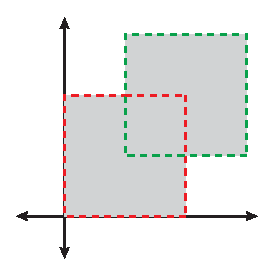
\includegraphics[width=200pt]{images/product_topology/product_sets_r}\]

Although products of open sets will not work because they are not closed under unions, we can use products of open sets to construct our topology. Define the following: 
\begin{definition}
	Let $(X,F_x)$ and $(Y,F_y)$ be topological spaces. Then the set $\beta_{X\times Y}$ is defined by:
	\[\beta_{X\times Y} = \{A\times B:\,A\in F_x,\,B\in F_y\}\]
	and define:
	\[F_{X\times Y} = \left\{\cup_{i\in I} U_i:\,I \text{ is some index set, and }U_i\in \beta_{X\times Y}\right\}\]
\end{definition}
In other words, $\beta_{X\times Y}$ is the set of products of an open set in $X$ and an open set in $Y$, and $F_{X\times Y}$ is the set of unions of elements in $\beta_{X\times Y}$. The motivation for defining our sets this way is that we want $F_{X\times Y}$ to be a topology on $X\times Y$ and for $\beta$ to be its basis. We will now verify this claim with the following \emph{small fact}: 
\begin{theorem}
	If $(X,F_x)$ and $(Y,F_y)$ are topological spaces, the space $(X\times Y,F_{X\times Y})$ is a topological space with basis $\beta_{X\times Y}$. 
\end{theorem}
\begin{proof}
	We will apply our basis theorem; i.e. we want to show that 
	\begin{enumerate}
		\item $\bigcup_{U\in \beta_{X\times Y}} U = X \times Y$ 
		\item Given $B_1,B_2\in\beta_{X\times Y}$, for each $x\in B_1\cap B_2$, there exists $B_3\in B_{X\times Y}$ such that $x\in B_3\subseteq B_1\cap B_2$. 
	\end{enumerate}
	
	For the first statement, we know that $X\in F_x$ and $Y\in F_y$ by definition of a topology so that $X\times Y\in \beta_{X\times Y}$. It follows then that because each $U\in \beta_{X\times Y}$ is subset of $X\times Y$:
	\[X \times Y \subseteq \bigcup_{U\in \beta_{X\times Y}} U \subseteq X\times Y\]
	so that $X\times Y = \bigcup_{U\in \beta_{X\times Y}} U$, as desired.
	
	For the second statement, let $B_1,B_2\in \beta_{X\times Y}$ and let $(x,y)\in B_1\cap B_2$. Then by definition of $\beta_{X\times Y}$, there exist $U_1,U_2\in F_x$ and $V_1,V_2\in F_y$ such that $B_1\cap B_2 = (U_1\times V_1)\cap (U_2\times V_2)$. 
	
	Our aim is to find $B_3\in \beta_{X\times Y}$ such that $B_3$ contains $(x,y)$ and $B_3\subseteq B_1\cap B_2$, so define:
	\[B_3 = (U_1\cap U_2) \times (V_1\cap V_2).\]
	Thus $U_1,U_2\in F_x\Rightarrow U_1\cap U_2\in F_x$ by the closure of topologies under finite intersections and similarly, $V_1\cap V_2\in F_y,$ so $B_3\in \beta_{X\times Y}$. Since $(x,y)\in (U_1 \times V_1)\cap (U_2\times V_2)$, then $(x,y)\in (U_1\times V_1)$ and $(x,y)\in (U_2\times V_2)$. Therefore, $x\in U_1,U_2$ and $y\in V_1,V_2$, so $x\in U_1\cap U_2$, and $y\in V_1\cap V_2$. It immediately follows by the definition of the intersection of sets that:
	\[(x,y) \in (U_1\cap U_2)\times (V_1\cap V_2) = B_3\]
	
	The only thing left to show is that $B_3\subseteq B_1\cap B_2$. To that end, let $(a,b)\in B_3$. Then $a\in U_1\cap U_2$ and $b\in V_1\cap V_2$ by definition of $B_3$. It follows that:
	\[a\in U_1,U_2 \text{ and } b\in V_1,V_2 \Rightarrow (a,b)\in U_1\times V_1 \text{ and } (a,b)\in U_2 \times V_2 \Rightarrow a\in (U_1\times V_1)\cap (U_2\times V_2).\]
	Therefore, $(a,b)\in B_1\cap B_2$ so that $B_3\subseteq B_1\cap B_2$ because $(a,b)$ is an arbitrary element of $B_3$. 
	
	Therefore, $\beta_{X\times Y}$ satisfies the hypotheses of our basis theorem, so the set of unions of elements of $\beta_{X\times Y}$, $F_{X\times Y}$, is a topology for $X\times Y$ and $\beta_{X\times Y}$ is a basis for the topology $F_{X\times Y}$. 
\end{proof}

We have successfully devised a topology for product spaces as unions of products of open sets.

\subsection{Examples}
\begin{example}
	The set $S^1 \times [0,1]$ looks like a cylinder! What kinds of sets are open in the cylinder? A particular example is an open disc projected on the face of the cylinder and unions thereof. 
\end{example}
\[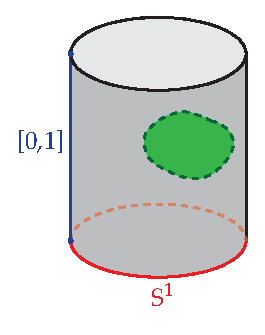
\includegraphics[width=100pt]{images/product_topology/s1_times_i}\]

\begin{example}
	The set $S^1 \times S^1$ looks like a torus! What kinds of sets are open in the torus? Similar to the previous example, open discs projected onto the torus surface are examples of open sets in $S^1\times S^1$.  In the picture, one copy of $S^1$ is red and one is green; they determine a torus.
\end{example}

\[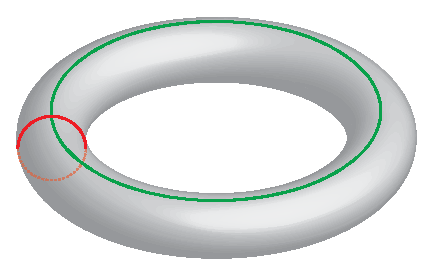
\includegraphics[width=160pt]{images/product_topology/s1_times_s1}\]

\begin{example}
	The set $S^1 \times S^1 \times S^1$ is actually a 3-torus! 
\end{example}

Not every space is a product of more than one space. For example the sphere $S^2$ is not a product of more than one space. An intuitive (non-rigorous) justification is that the natural axes of a sphere are the great circles; however, every pair of distinct great circles intersect twice which makes it hard to define a coordinate system on the sphere.

\subsection{The Product Projection Map}

Now that we have a product topology to impose on product spaces, we want a way to relate the product topology to the topologies of the constituent spaces. In order to do so, we will define the projection maps as follows: 
\begin{definition}
	Let $(X,F_x)$ and $(Y,F_y)$ be topological spaces and create $X\times Y$ endowed with the product topology $F_{X\times Y}$. Define $\pi_X: (X\times Y,F_{X\times Y}) \to (X,F_x)$ and $\pi_Y:(X\times Y,F_{X\times Y}) \to (Y,F_y)$ by:
	\[\pi_X((x,y)) = x \qquad \pi_Y((x,y)) = y.\]
	The map $\pi_X$ is the projection onto $X$ and $\pi_Y$ is the projection onto $Y$. 
\end{definition}

A small fact which we will derive now is that the product projection maps are continuous: 
\begin{theorem}
	Let $(X,F_X)$ and $(Y,F_Y)$ be topological spaces and $(X\times Y,F_{X\times Y})$ be their product with the induced product topology. Then the projection maps $\pi_X$ and $\pi_Y$ onto $X$ and $Y$ are continuous. 
\end{theorem}
\begin{proof}
	Suppose $O\subseteq X$ and $O\in F_x$. We see that $\pi^{-1}(O) = O\times Y \in F_{X\times Y}$. Therefore, the preimage of any open set in $X$ under $\pi_X$ is open in $X\times Y$ with the product topology. A similar argument shows that $\pi_Y$ is continuous. 
\end{proof}

Recall that the quotient projection map is \emph{not necessarily} an open map. It turns out that the product projection map \emph{is} an open map. Accidentally assuming that the quotient map is open is a very common mistake that one should be aware of! We will now prove that the product projection map is open: 
\begin{theorem}
	Let $(X,F_X)$ and $(Y,F_Y)$ be topological spaces and $(X\times Y,F_{X\times Y})$ be their product with the induced product topology. Then the projection maps $\pi_X$ and $\pi_Y$ onto $X$ and $Y$ are open. 
\end{theorem}
\begin{proof}
	Let $O = U\times V$ such that $U \in F_x$ and $V\in F_y$ and $O\in \beta_{X\times Y}$. Therefore:
	\[\pi_X(O) = U\in F_x\]
	So if $C$ is some collection of sets in $\beta_{X\times Y}$, then:
	\[\bigcup_{V\in C}V\]
	is an arbitrary element of $F_{X\times Y}$ by the definition of a basis and:
	\[\pi_X\left( \bigcup_{V\in C}V \right) = \bigcup_{V\in C} \pi_X(V)\]
	which is open because the preceding statments indicate that $V\in \beta_{X\times Y} \Rightarrow \pi_X(V)\in F_X$. Consequently, the image of the arbitrary open set in $(X\times Y, F_{X\times Y})$ is a union of open sets in $(X,F_x)$ and is thus open.
	
	The proof is similar for $\pi_Y$. 
\end{proof}

\subsection{Using Bases More Effectively}

In metric spaces, open balls are bases for the metric topology. By proving properties about open balls, we were able to say they apply to the entire set. We would like to prove the following \emph{important tiny lemma} so that we can use bases in topological spaces like open balls in metric spaces: 
\begin{lemma}
	Let $(X,F_x)$ be a topological space with basis $\beta$. If $W\subseteq X$ then $W\in F_x$ if and only if for all $p\in W,$ there exists $B_p\in\beta$ such that $p\in B_p\subseteq W$. 
\end{lemma}
\begin{proof}
	\begin{itemize}
		\item[$(\Rightarrow)$] Suppose $W\in F_x$. Let $p\in W$. Since $W\in F_x$, for some index set $I$:
		\[W = \bigcup_{i\in I}B_i \qquad \forall i\in I,\,B_i\in \beta\]
		because every element of a topology can be written as a union of basis elements. Therefore, by definition of the union, $p\in W$ implies that there exists $i_p\in I$ such that $p\in B_{i_p}$, and $B_{i_p}\subseteq W$. If we let $B_p = B_{i_p}$, we are finished.
		
		\item[$(\Leftarrow)$]
		
		Suppose that for all $p\in W$, there exists $B_p\in \beta$ such that $p\in B_p\subseteq W$. We want to show that $W\in F_x$. We see that:
		\[V = \bigcup_{p\in W}B_p\subseteq W\]
		because each of the constituent $B_p\subseteq W$, and every $p\in W$ is an element of $B_p$, so the union of $B_p$ over $p\in W$, contains every $p\in W$. Consequently, $V\subseteq W \Rightarrow V=W$. Since $\beta$ is a basis and $V$ is a union of basis elements, $V\in F_x \Rightarrow W\in F_x$. 
	\end{itemize}
\end{proof}

In other words, if we have a topological space with a basis, then every point in an open set $U$ is an element of a basis element contained in $U$, giving us a structure very similar to the metric topology.

\subsection{Finding and Constructing Continuous Maps to Product Spaces}

Now that we have product spaces and have addressed their basic topological properties, we would like a way to easily find and construct continuous maps to the product space. To that end we introduce the following \emph{important lemma}: 
\begin{lemma}
	Let $(X,F_X),(Y,F_Y)$ and $(A,F_A)$ be topological space and let $(X\times Y,F_{X\times Y})$ be the product space of $X,Y$ with the induced product topology. Suppose $f:A\to X$ and $g:A\to Y$ and define
	\[h:A\to(X\times Y) \qquad \text{ by } \qquad h(a) = (f(a),g(a)),\]
	then $h$ is continuous if and only if $f,g$ are continuous. 
\end{lemma}
\begin{proof}
	\begin{itemize}
		\item[$(\Rightarrow)$] Suppose $h$ is continuous: then we see that:
		\[f = \pi_X \circ h \qquad g = \pi_Y \circ h\]
		so $f,g$ are continuous because they are compositions of continuous functions. 
		\item[$(\Leftarrow)$] Suppose that $f$ and $g$ are continuous. We prove that the preimage of every basis element under $h$ is open. From a theorem we proved some time ago, this shows that $h$ is continuous.
		
		Let $U\times V\in \beta_{X\times Y}$. Then $U\in F_X$ and $V\in F_Y$. Since $f$ and $g$ are continuous, $f^{-1}(U)\in F_A$ and $g^{-1}(V)\in F_A$. Then 
		\begin{align*}
			h^{-1}(U\times V) &= \{a\in A\ |\ h(a)\in U\times V\}\\
			&= \{a\in A\ |\ (f(a), g(a))\in U\times V\}\\
			&= \{a\in A\ |\ f(a)\in U, g(a)\in V\}\\
			&= f^{-1}(U)\cap g^{-1}(V) 
		\end{align*}
		Then $h^{-1}(U\times V)$ is the intersection of two open sets, hence it is open. Therefore, $h$ is continuous. 
	\end{itemize}
\end{proof}

The following example illustrates how this lemma makes it very easy to define continuous functions to the product space: 
\begin{example}
	Suppose $f:\R\to\R$ and $g:\R\to\R$ with $f(x) = x^2+3x$ and $g(x) = \sin(x)$. Then the map $h:\R\to\R^2$ defined by $h(x) = (x^2+3x, \sin(x))$ is continuous because $f,g$ are. 
\end{example}

\subsection{Relating Products to Subspaces} 
\begin{smallfact}
	Let $(X, F_X)$ and $(Y, F_Y)$ be topological spaces with subspaces $(A, F_A)$ and $(B, F_B)$ respectively. Let $F_S$ denote the subspace topology on $A\times B\subseteq X\times Y$ and let $F_{A\times B}$ denote the product topology on $A\times B$. Then $F_S = F_{A\times B}$. 
\end{smallfact}
This means that we can either look at $A\times B$ as a subspace of $X\times Y$, then induce the subspace topology, or we can induce the subspace topologies on $A$ and $B$, then take the cross product. Essentially, taking the cross product and creating subspaces ``commute.'' 
\begin{proof}
	We start by reviewing which sets are open under each topology:
	\[ F_S = \{ (A\times B)\cap U\ |\ U\in F_{X\times Y} \}\]
	\[ F_{X\times Y} = \text{unions of sets of the form } U\times V\text{, with } U\in F_A, V\in F_B \]
	
	Let $U\cap(A\times B)\in F_S$. Then
	\[ U\cap(A\times B) = \bigcup_{i\in I} (U_i\times V_i)\cap (A\times B) \qquad\qquad\text{(where }\forall i\in I, U_i\in F_X, V_i\in F_Y)\]
	Then 
	\begin{align*}
		U\cap(A\times B) &= \bigcup_{i\in I} (U_i\times V_i)\cap (A\times B)\\
		&= \{ (x,y)\in A\times B\ |\ (x,y)\in U_{i'}\times V_{i'}\text{ for some }i'\in I \} \\
		&= \{ (x,y)\in X\times Y\ |\ x\in U_{i'}\cap A, y\in V_{i'}\cap B\text{ for some }i'\in I\} \\
		&= \bigcup_{j\in J} (U_j\cap A)\times (V_j\cap B)\qquad\qquad\text{ for some index set} J \}\\
		&\in F_{X\times Y} 
	\end{align*}
	The same argument run backwards shows that $F_{X\times Y}\subseteq F_S$.
	
	Therefore, $F_{S} = F_{X\times Y}$. 
\end{proof}

\subsection{Products and Quotient Spaces} Taking products and quotients does not ``commute'' in the same way that taking products and subspaces does. We demonstrate a (lengthy) counterexample to this idea.

Consider $\R$ with the usual topology, with $x\sim Y$ iff $x=y$ or $x,y\in \N$. This looks something like a ``sideways infinite flower.'' 

\[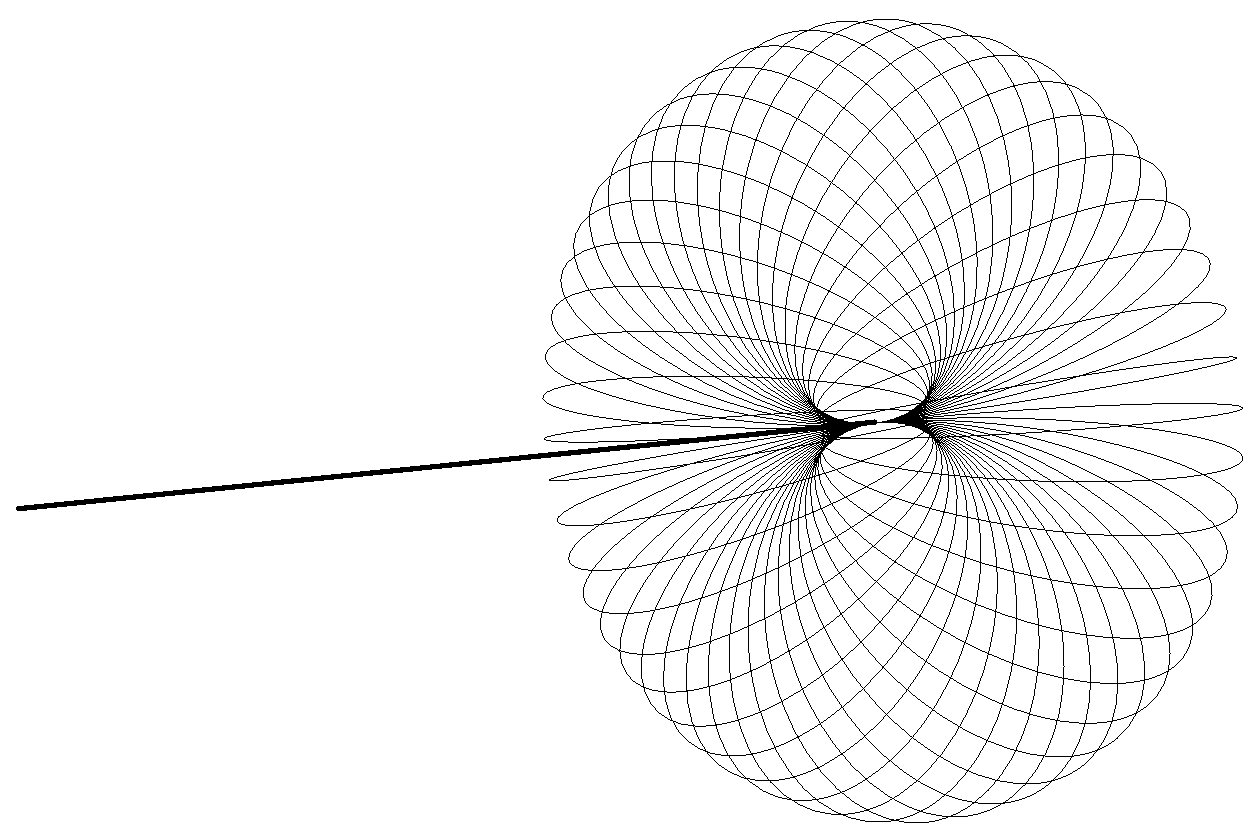
\includegraphics[width=300pt]{images/product_topology/sideways_infinite_flower}\]

 If a set open in $\R/\sim$ contains a (``the'') natural number, then its preimage must contain every natural number, so it must contain an open interval about ``the'' natural number in every direction (all infinity of them). 

More formally, let $\pi:\R\to\R/\sim$ be the projection map. Let $id_\Q:\Q\to\Q$ be the identity map, where each copy of $\Q$ has the usual topology. Note that $id_\Q$ is a quotient map (where $\sim$ is `='). 

Now, consider $\pi\times id_\Q:\R\to\Q\to(\R/\sim)\times\Q$ by $(\pi\times id_\Q)(x,y) = (\pi(x), i(y))$. We claim that $\pi\times id_\Q$ is not a quotient map. To prove this, we show that the product topology on $(\R/\sim)\times\Q$ is not the same as the quotient topology
\[ \{ U\in (\R/\sim)\times\Q\ |\ (\pi\times id_\Q)(U)\in F_{\R\times\Q} \} \]
To do this, let's find some $U' \in F_{\pi \times i}$ such that $U' \notin F_{(\R/\sim) \times \Q}$. We want to construct $U'$ as a union.

For all $n\in \N$ define $U_n$ to be the interior of the region of $\R\times\Q$ bounded by the vertical lines $n-\frac{1}{4}$ and $n+\frac{1}{4}$ and above and below by the lines through $(n, \frac{\sqrt{2}}{n})$ with slope $\pm 1$. Each one of these sets has a vertical line through the natural number.

So $\forall n \in \N, \{n\}\times \Q \subseteq U_n$. Observe that $\forall n\in \N, U_n \in F_{\R\times\Q}$ (it is an interior, so it is open).

Let $\bigcup_{n \in\N} U_n \in F_{\R\times\Q} \qquad$ (also open in $\R\times\Q$ because it is a union).

Let $U' = (\pi \times i)(U).$ This will glue together the strips along the vertical lines with $\R$ coordinates in $\N$. This can be pictured as a fan.
\[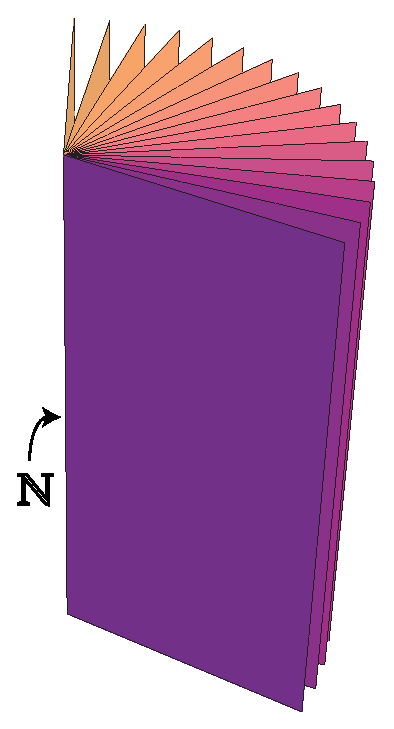
\includegraphics[width=400pt]{images/product_topology/sideways_infinite_fan}\]

Claim: $U' \in F_{\pi \times i}$

\proof: $(\pi \times i)^{-1}(U') = U$ and $U$ is a union of $U_n 's$

Therefore, by definition, $U'\in F_{\pi\times i}$.

\mbox{ }

Claim: $U'\not\in F_{(\R/\sim) \times \Q}$.

\proof: Let $([n],0) \in U'$. Suppose $\exists W \in F_{\R/\sim}$ and $V \in F_{\Q}$ such that $([n], 0)\in W \times V \subseteq U'$.

Then $\pi^{-1}(W) \in F_{\R}$ and of course $i^{-1}(V) = V$.

So $\pi^{-1}(W) \times V$ is open in $\R\times \Q$ such that $\pi^{-1}(W) \times V \subseteq (\pi \times i)^{-1}(U') = U$.

Also, $\pi^{-1}(W)$ is open in $\R$ and contains $\N$ and $V$ is open in $\Q$ and contains $\{0\}$.

So $\exists \delta >0$ such that $(-\delta, \delta) \cap \Q \subseteq V$. There exists an $n\in \N$ such that $\delta > \frac{\sqrt{2}}{n}$. $\pi^{-1}(W)$ is open in $\R$, so it's on the x-axis.

So $\exists \epsilon >0$ such that $(n-\epsilon, n+\epsilon)\subseteq \pi^{-1}(W)$.

So the interval $(n-\epsilon, n+\epsilon)\times (-\delta, \delta)\subseteq \pi^{-1}(W)\times V$. So $\epsilon < \frac{1}{4}$ from our previous definition of $U_n$.

Let $x = n + \frac{\epsilon}{2}$. Question: Where does $x = n + \frac{\epsilon}{2}$ meet the boundaries of $U_n$? It meets at $y = \frac{\sqrt{2}}{n} \pm \frac{\epsilon}{2}$.

$\exists y \in \Q$ such that $\frac{\sqrt{2}}{n} - \frac{\epsilon}{2} < y < \frac{\sqrt{2}}{n} + \frac{\epsilon}{2}$.

So $(x,y) \notin U_n$ and $\forall m\neq n, (x,y)\notin U_m$ since $(x,y) \in (n-\epsilon, n+\epsilon)\subseteq (n-\frac{1}{4}, n+\frac{1}{4}$.

But $(x,y) \in (n-\epsilon, n+\epsilon) \times (-\delta, \delta) \subseteq \pi^{-1}(W) \times V \subseteq U$ $\Rightarrow (x,y) \notin U$. Therefore we have a contradiction.

$\therefore U' \notin F_{(\R/\sim)\times \Q}$

So we have shown that $F_{\pi\times i} \neq F_{(\R/\sim) \times \Q}$.

\subsection{Infinite Products} We would of course like to be able to generalize this to deal with infinite products. Initially, we may simply want to define such products as follows: $X_1$x$X_2$x...$=\{(x_1,x_2,...)|x_i \in X_i \forall i \in \N \}$. However, such a definition limits us to countable products, so we look more generally.
\begin{definition}
	$j \in J$, let $X_j$ be a set. Define the product $\Pi_{j \in J} X_j = \{f:J \rightarrow \cup_{j \in J}X_j|f(j) \in X_j\}.$ We refer to $f(j)$ as the $j^{th}$ coordinate of the point $f$. 
\end{definition}
\begin{example}
	Suppose $J = \{1,2\}$. Then $\Pi_{j\in \{1,2\}}X_j = \{f: \{1,2\} \rightarrow X_1\cup X_2|f(j) \in X_j\} = \{(f(1),f(2))|f(j) \in X_j\}=\{(x_1,x_2)|x_j \in X_j\} = X_1$ x $X_2.$ Thus we see that this definition agrees with our previous definition for finite products. 
\end{example}
\begin{example}
	Consider $\Pi_{j \in \R}\{1,2\}$. By definition this is equivalent to $\{f: \R \rightarrow \{1,2\}| f(j) \in \{1,2\}, j \in \R\}$, which precisely correspond to subsets of $\R$ if we simply think of the preimage of $1$ under $f$ as the elements in the set and the preimage of $2$ under $f$ as those elements outside the set. Commonly this product is then denoted by $\{1,2\}^{\R}$. 
\end{example}

Now we wish to define a topology on these products which, as in example $1$, agrees with our prior definition for a product of two sets if the indexing set $J = \{1,2\}$. Perhaps the most natural way of doing this is to define the following basis: 
\begin{center}
	$\beta_{\Box} = \{\Pi_{j \in J} U_j|U_j \in F_j\}$, where $X_j$ has topology $F_j$.
	
	$F_{\Box} = \{$Unions of elements of $\beta_{\Box}\}.$ 
\end{center}
This topology is not what we desire, but is a topology, aptly named the box topology on the product.
\begin{example}
	The product topology on $\Pi_{j \in J}X_j$ is given by the basis $\beta_{\Pi} = \{\Pi_{j \in J}U_j|U_j = X_j$ for all but finitely many $j$ and $\forall j \in J, U_j \in F_j \}$. 
\end{example}

Remarks: 
\begin{enumerate}
	\item $\beta_{\Pi} \subseteq \beta_{\Box}$ 
	\item Both are bases for topologies on the product. 
\end{enumerate}
\begin{definition}
	Define the projection map $\pi_j : \Pi_{j \in J}X_j \rightarrow X_j$ by $\pi(f) = f(j)$. 
\end{definition}
\begin{lemma}
	For all $j \in J$, Suppose $(X_j, F_j)$ is a topological space. Then $\pi_j$ as defined above is continuous for all $j \in J$. 
\end{lemma}
\begin{proof}
	Let $j_{0} \in J$ and consider $U \in F_{j_{0}}$. We wish to show that $\pi_{j_{0}}^{-1}(U) \in F_{\Pi}$. Note that $\pi_{j_{0}}^{-1}(U) = \{f \in \Pi_{j \in J}X_j | \pi_{j_{0}}(f) \in U\} = \{f \in \Pi_{j \in J}X_j | f(j_{0}) \in U\} = \{f \in \Pi_{j \in J}X_j | f(j_{0}) \in U, \forall j \neq j_{0} f(j) \in X_{j}\}= \Pi_{j \in J} U_j$ such that $U_{j_{0}} = U$ and $\forall j \neq j_{0}, U_j = X_j$.\\
	It then follows from definitions that $\pi_{j_{0}}^{-1}(U) \in \beta_{\Pi} \subseteq F_{\Pi}$ so the projection map is continuous. 
\end{proof}

We now prove an Important Lemma for Infinite Products. 
\begin{lemma}
	Let $(X_j,F_j)$ and $(Y,F_Y)$ be topological spaces for all $j \in J$. Moreover, for each such j let $g_j : Y \rightarrow X_j$ be a function. Define $h: Y \rightarrow \Pi_{j \in J}X_j$ by: $h(y) = f$ such that $\forall j \in J, f(j) = g_{j}(y)$. Then $h$ is continuous if and only if $g_j$ is continuous for all $j \in J$. 
\end{lemma}
\begin{proof}
	\begin{itemize}
		\item[($\Rightarrow$)] Suppose $h$ is continuous and let $j \in J$. Then $\pi_j \circ h = g_j$. Thus $g_j$ is the composition of continuous functions and must itself be continuous. 
		\item [($\Leftarrow$)] Suppose that $g_j$ is continuous for all $j \in J$. Let $U \in \beta_{\Pi}.$ We wish to show that $h^{-1}(U) \in F_{Y}$.
		
		Note that $h^{-1}(U) = \{y \in Y | h(x) \in U\}$ As an open set in the product topology, $U = \Pi_{j \in J}U_j$ where $U_j \in F_j$. Thus, $h^{-1}(U) = \{y \in Y | h(x) \in \Pi_{j \in J}U_j\} = \{f \in \Pi_{j \in J}U_j$ such that $\forall j \in J, f(j) = g_{j}(y)\} = \{y \in Y | g_{j}(y) \in U_j\} = \{y \in Y | y \in g_{j}^{-1}(U_j) \forall j \in J\} = \cap_{j \in J} U_j$.
		
		Since $g_j$ is continuous for all $j$, $g_{j}^{-1}(U_j)$ is open in $Y$ for all $j$. Also, by definition of the product topology, $U_j = X_j$ for all but at most finitely many $j$. Thus, $g_{j}^{-1}(U_j) = Y$ for all but at most finitely many $j$. It follows that the intersection $\cap_{j \in J} U_j$ is a finite intersection of open sets since removing all trivial indices will not change the intersection. Thus, $h^{-1}(U) \in F_Y$ so $h$ is continuous, completing the proof. 
	\end{itemize}
\end{proof}
